\documentclass{report}
\usepackage[utf8]{inputenc}
\usepackage{amsmath}
\usepackage{amssymb}
\usepackage{amsthm}
\usepackage{pgfplots}
\usepackage{tikz}
\usepackage{float}
\usepackage[danish]{babel}
\usepackage[margin=1.2in]{geometry}
\usepackage{xcolor}
\usepackage{pdfpages}
\usepackage{csquotes}

\renewcommand{\thesubsection}{\thesection.\alph{subsection}}

\title{Opgave 2, uge 2}
\author{Sebastian Winkelmann}
\date{23. september 2019}

\begin{document}
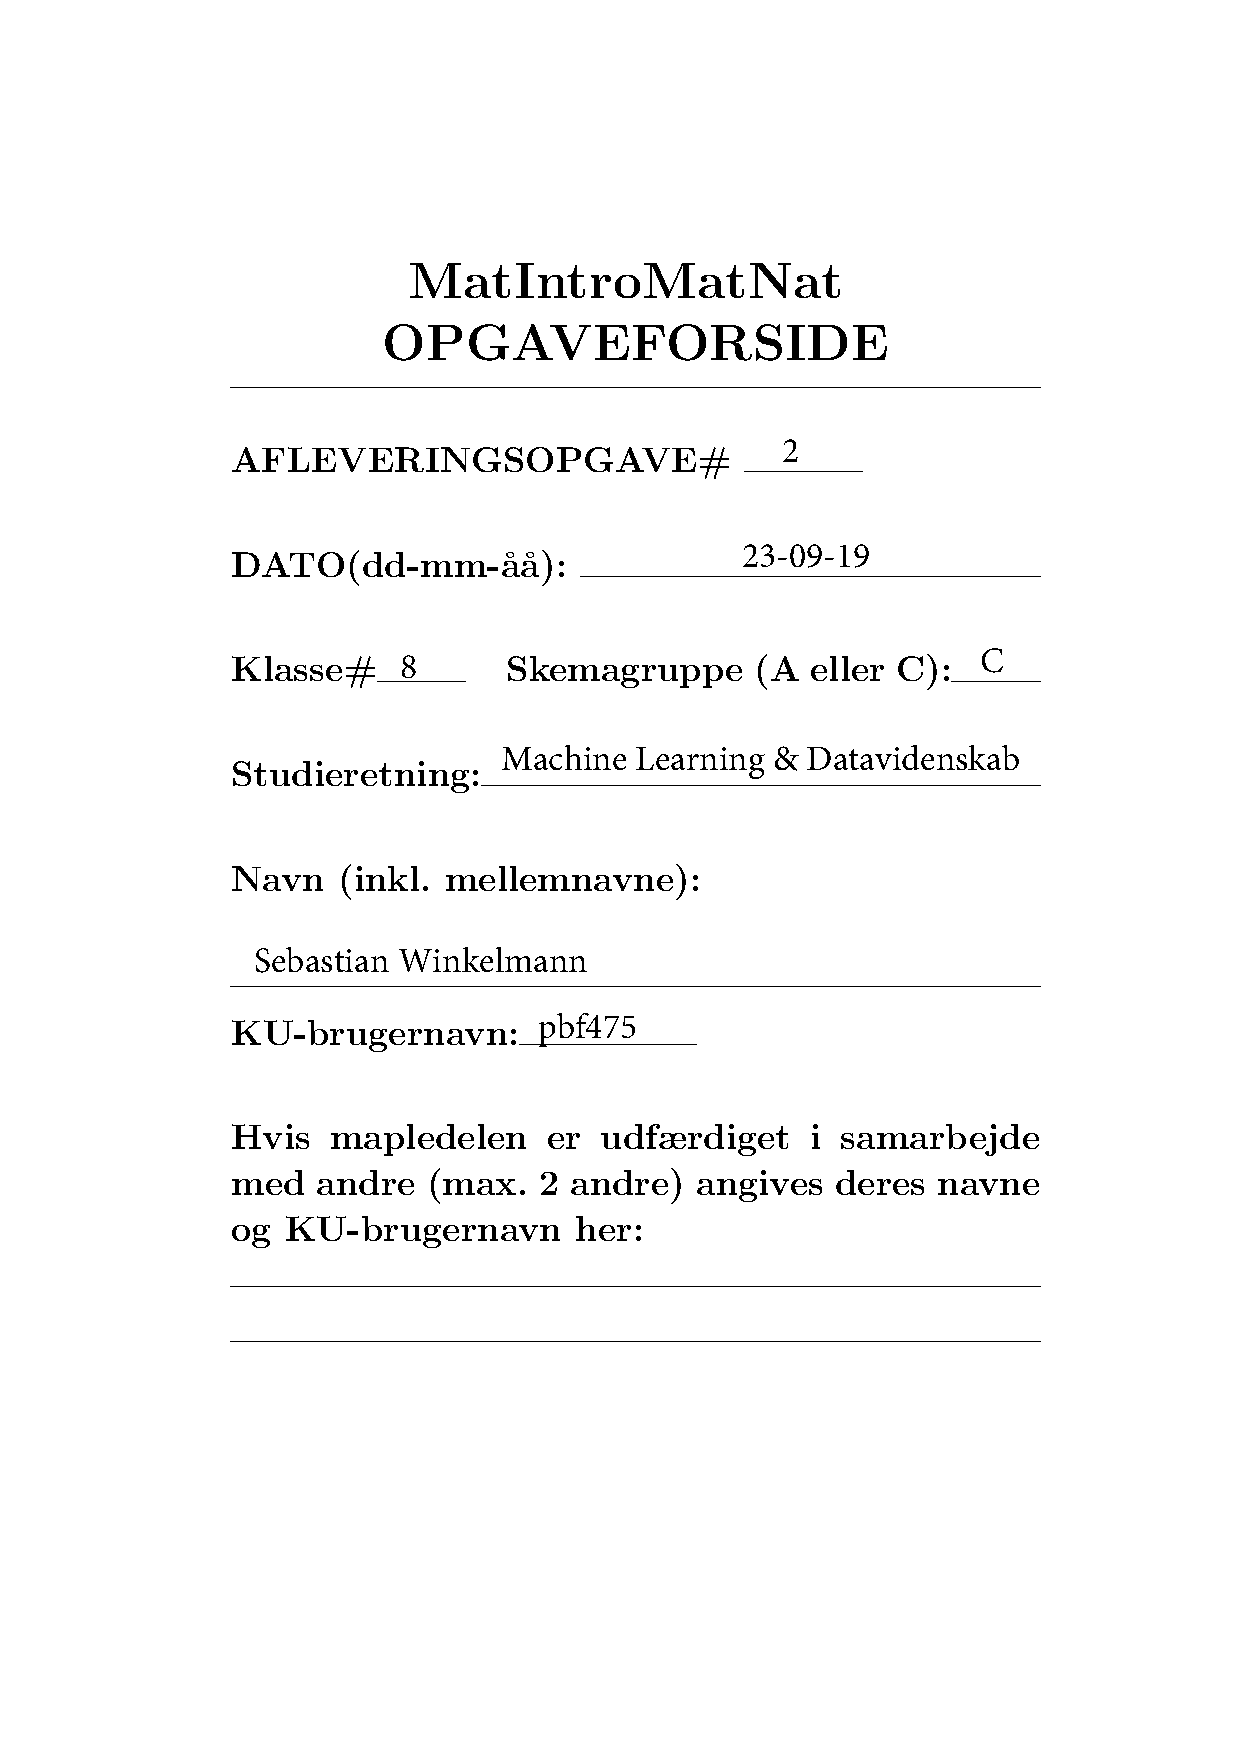
\includepdf{forside.pdf}
\setcounter{chapter}{2}
\section{}
$$f(x)=\frac{1}{x}-\frac{\cos{x}}{\sin{x}}$$for alle $x\in\mathbb{R}$ med $x\neq n\pi,\, n\in\mathbb{Z}$.
\subsection{Grænseværdien for $f$ når $x\to0^+\land\pi^-$}
Først i Maple
\begin{figure}[H]
    \centering
    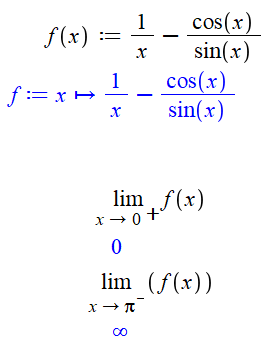
\includegraphics[width=0.333\textwidth]{limit21.png}
    \caption{Udregninger i Maple}
    \label{fig:limit21}
\end{figure}
Lad os udregne det. Først når $x\to0^+$
\begin{align*}
    \lim_{x\to0^+}f(x)&=\lim_{x\to0^+}\frac{1}{x}-\frac{\cos{x}}{\sin{x}}\\
    \lim_{x\to0^+}f(x)&=\lim_{x\to0}\frac{\sin{x}-x\cos{x}}{x\sin{x}}\end{align*}
Vi har her en grænseværdi som \enquote{0/0}-udtryk. Vi bruger L'Hôpitals regel
\begin{align*}
    \lim_{x\to0^+}\frac{(\sin{x}-x\cos{x})'}{(x\sin{x})'}&=\lim_{x\to0^+}\frac{\cos{x}-1\cos{x}+x\sin{x}}{1\sin{x}+x\cos{x}}\\
    &=\frac{\lim_{x\to0^+}x\sin{x}}{\lim_{x\to0^+}1\sin{x}+x\cos{x}}\\
    &=\frac{0}{0+0}
\end{align*}
Vi har her en grænseværdi som \enquote{0/0}-udtryk. Vi bruger L'Hôpitals regel
\begin{align*}
    \lim_{x\to0^+}\frac{(x\sin{x})'}{(\sin{x}+x\cos{x})'}&=\lim_{x\to0^+}\frac{\sin{x}+x\cos{x}}{\cos{x}+\cos{x}-x\sin}\\&=\lim_{x\to0^+}\frac{\sin{x}+x\cos{x}}{2\cos{x}-x\sin{x}}\\
    &=\frac{0+0\cdot1}{2\cdot1-0\cdot0}=\frac{0}{2}=0
\end{align*}
Således findes der en værdi, og vi har gennem L'Hôpitals regel fundet at\begin{equation}
    \lim_{x\to0^+}\frac{1}{x}-\frac{\cos{x}}{\sin{x}}=0
\end{equation}
Nu for $x\to\pi^-$:
\begin{align*}
    \lim_{x\to\pi^-}f(x)&=\lim_{x\to\pi^-}\frac{1}{x}-\frac{\cos{x}}{\sin{x}}=\lim_{x\to\pi^-}\frac{\sin{x}-x\cos{x}}{x\sin{x}}\\
    &=\frac{\lim_{x\to\pi^-}\sin{x}-x\cos{x}}{\lim_{x\to\pi^-}x\sin{x}}
\end{align*}
Vi bemærker at der i nævneren vil stå $\pi\sin{\pi}\to0$, mens der i tælleren vil stå $\sin{\pi}-x\cos{x}\to0-\pi(-1)$. Da $\lim_{x\to0}\frac{1}{x}=\infty$ og $\sin{x}$ er en kontinuert, periodisk funktion for hvilket det gælder at $\sin{x}>0,\forall x\in(2n\pi, (2n+1)\pi)$, hvor $n\in\mathbb{Z}$, ved vi at $\frac{\sin{x}-x\cos{x}}{x\sin{x}}$. Vi har altså at grænseværdien giver positiv uendelig.
\begin{equation}
    \lim_{x\to\pi^-}\frac{1}{x}-\frac{\cos{x}}{\sin{x}}=\infty
\end{equation}
\subsection{$f$ er strengt voksende}
Funktionens vækst kan findes ved funktionens afledede. Vi differentierer $f$.
\begin{align*}
    f'(x)&=\frac{d}{dx}\left(\frac{1}{x}-\frac{\cos{x}}{\sin{x}}\right)\\
    &=-\frac{1}{x^2}+\frac{1}{\sin^2{x}}
\end{align*}
Vi kan her se at alle alle led indeholder kvadreringer, hvor nævneren i hverken kan være negativ. For at $f'(x)>0$ når $x\in(n\pi,(n+1)\pi)\setminus0$ skal vi vise at $\frac{1}{\sin^2{x}}>\frac{1}{x^2}$. $|\sin{x}|<|x|$ medfører at dette nødvendigvis udsagn må være sandt. Det er hermed vist at $f$ er strengt voksende i intervallet:\begin{equation}
    f'(x)=\frac{1}{\sin^2{x}}-\frac{1}{x^2}>0,\forall x\in(n\pi,(n+1)\pi)
\end{equation}
\subsection{Bevis at $f(x)=0$ ikke har nogen løsninger i $(0,\pi)$, men præcis én løsning i $(\pi,2\pi)$}
Rent grafisk er der tale om et bevis for at $f$ ikke skærer $x$-aksen i intervallet $(0,\pi)$, men gør det præcist én gang i intervallet $(\pi,2\pi)$.
\begin{proof}
Vi har tidligere vist at $f$ er strengt voksende i intervallet $(n\pi,(n+1)\pi$, at $\lim_{x\to0^+}f(x)=0$ samt at $f(x)>0,\forall x\in(n\pi,(n+1)\pi)$. Vi kan benytte sidstnævnte til at vise værdiintervallet i \small{(hvor $n=0$)} $(0,\pi)$:$$f(x)>0,\forall x\in(0,\pi)$$Altså har $f(x)=0$ ingen løsninger i $(0,\pi)$. Lad os nu undersøge $f(x)=0$ i $(\pi,2\pi)$ ved at undersøge grænseværdierne for det lukkede interval $[\pi,2\pi]$. Vi kan udnytte vores resultater fra a), idet den dobbeltsidet grænseværdi har to løsninger med modsat fortegn og der er tale om en periodisk funktion (vi kan altså udnytte at der for $f$ gælder at $\lim_{x\to\pi^-}f(x)=-\lim_{x\to\pi^+}f(x)$ samt $\lim_{x\to\pi^-}f(x)=\lim_{x\to2\pi^-}f(x)$). Starter med $x\to\pi^+$:$$\lim_{x\to\pi^+}\frac{1}{x}-\frac{\cos{x}}{\sin{x}}=-\lim_{x\to\pi^-}\frac{1}{x}-\frac{\cos{x}}{\sin{x}}=-\infty$$Modsat har vi for $x\to2\pi^-$:$$\lim_{x\to2\pi^-}\frac{1}{x}-\frac{\cos{x}}{\sin{x}}=\lim_{x\to\pi^-}\frac{1}{x}-\frac{\cos{x}}{\sin{x}}=\infty$$
Ifølge skæringssætningen vil der for en kontinuerlig funktion $f:[a,b]\to\mathbb{R}$ hvor $f(a)=-f(b)$ findes der et tal $c\in(a,b)$ således at $f(c)=0$. Da vi ved at $\lim_{x\to\pi^+}f(x)<0<\lim_{x\to2\pi^-}f(x)$ og siden $f(a)<f(b),\forall a<b\in(\pi,2\pi)$ findes der én og kun én løsning til ligningen $f(x)=0$ i $x\in(\pi,2\pi)$
\end{proof}
\begin{figure}[H]
    \centering
    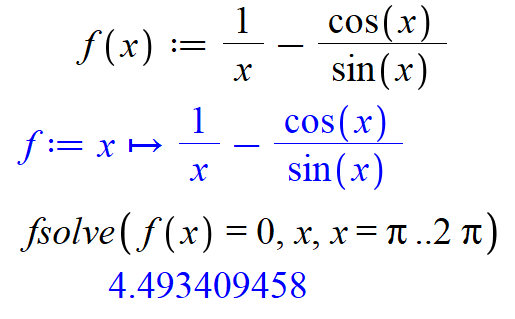
\includegraphics[width=0.33\textwidth]{21c.png}
    \caption{Løsning i Maple}
\end{figure}

\section{}
En funktion $f:\mathbb{R}\longrightarrow\mathbb{R}$ defineres ved$$f(x)=\begin{cases}\frac{1-x^2}{(x-1)(x-3)}&x\in(-\infty,1)\cup(3,\infty)\\x&x\in[1,3]\end{cases}$$
\subsection{Udsnit af grafen for $f$}
\begin{figure}[H]
    \centering
    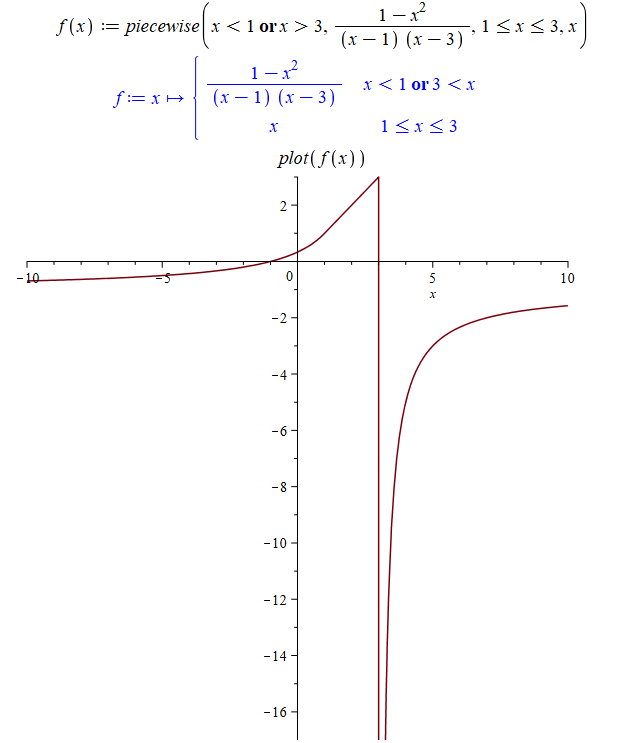
\includegraphics[width=0.5\textwidth]{22a.png}
\end{figure}

\subsection{$f$ differentiabel i $x=1$}
Da der for den stykvise definition gælder at $x=1\implies f(x)=x$, og $f(x)=x$ er differentiabel må $f'(1)=\frac{dx}{dx}
=1$ eksistere, og $f$ er derfor differentiabel i $x=1$. Vi kan desuden vise det ifølge definitionen og middelværdisætningen. Der gælder nemlig at hvis $g$ er en kontinuert funktion ved $x=c$ og differentiabel på begge sider af $x=c$, og hvis $\lim_{x\to c^-}g(x)=\lim_{x\to c^+}g(x)=L$ samt grænseværdien $\lim_{x\to c^-}g'(x)=\lim_{x\to c^+}g'(x)=Q$, da må $g$ være differentiabel i $x=c$ med $g'(c)=L$.\\
Differentialkvotienten for $f=\frac{1-x^2}{(x-1)(x-3)}$ kan findes ved $$\left(\frac{1-x^2}{(x-1)(x-3)}\right)'=\frac{4}{(x-3)^2}$$
\begin{align*}
    \lim_{x\to1^+}f'(x)&=\lim_{x\to1^+}1=1\\
    \lim_{x\to1^-}f'(x)&=\lim_{x\to1^-}\frac{4}{(x-3)^2}\\
    &=\frac{4}{(1-3)^2}=\frac{4}{(-2)^2}=\frac{4}{4}=1
\end{align*}{}
Og
\begin{align*}
    \lim_{x\to1^+}f(x)&=\lim_{x\to1^+}x=1\\
    \lim_{x\to1^-}f(x)&=\lim_{x\to1^-}\frac{1-x^2}{(x-1)(x-3)}\\
    &=\lim_{x\to1^-}\frac{(1^2-x^2)}{(x-1)(x-3)}\\
    &=\lim_{x\to1^-}\frac{-(x-1)(x+1)}{(x-1)(x-3)}\\
    &=\lim_{x\to1^-}\frac{-(x+1)}{(x-3)}\\
    &=\frac{-2}{-2}=1
\end{align*}{}\newpage
\section{(iii)}
Betragt funktionen $f(x)=x(\ln{(x+1)}-\ln{x}),x>0$
\subsection{Tegn grafen for $0<x\leq100$ og gæt på $\lim_{x\to\infty}f(x)$}
\begin{figure}[H]
    \centering
    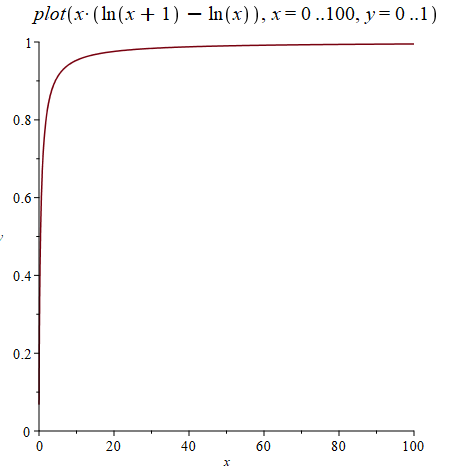
\includegraphics[width=0.5\textwidth]{31.png}
\end{figure}
Umiddelbart konvergerer $f(x)$ mod $1$, således at $V_f=\{y\in\mathbb{R}|0<x<1\}$ og $\lim_{x\to\infty}f(x)=1$
\subsection{Beregning af $f(10^n)$ for $n=1,\ldots,10$}
\begin{figure}[H]
    \centering
    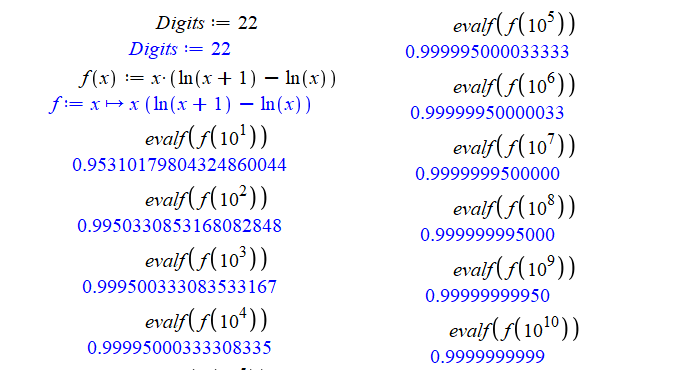
\includegraphics[width=0.8\textwidth]{32.png}
\end{figure}
Det er her meget tydeligt at $f$ danner asymptote med $y=1$, og grænseværdien er $\lim_{x\to\infty}f(x)=1$.
\subsection{$\lim_{x\to\infty}f(x)$}
Da $\ln{x}$ er asymptotisk med $e$, og man for meget høje $x$ har en meget lille differens. Der gælder nemlig at $\lim_{x\to\infty}\ln{(x+1)}=\lim_{x\to\infty}\ln{x}$, hvorfor differensen må være $\lim_{x\to\infty}\ln{(\frac{1}{x}+1)}=0$. Vi kan desuden hurtigt se at $x=\frac{1}{1/x}$. Vi kan altså omskrive grænseværdien af $f$ når $x\to\infty$ til et \enquote{$0/0$}-udtryk:
\begin{align*}
    \lim_{x\to\infty}f(x)&=\lim_{x\to\infty}x(\ln{(x+1)}-\ln{x})\\
    &=\lim_{x\to\infty}\frac{\ln{(x+1)}-\ln{x}}{1/x}\\
    \text{L'Hôpitals regel benyttes:}\\
    \lim_{x\to\infty}\frac{(\ln{(x+1)}-\ln{x})'}{(1/x)'}&=\lim_{x\to\infty}\frac{\frac{1}{x+1}-\frac{1}{x}}{-\frac{1}{x^2}}\\
    &=\lim_{x\to\infty}\frac{x(x-1-x)}{-(x+1)}\\&=\lim_{x\to\infty}\frac{x}{x+1}\\
    &=\lim_{x\to\infty}\frac{1}{1+1/x}\\
    &=\lim_{x\to\infty}\frac{1}{1+0}\\
    \lim_{x\to\infty}f(x)&=1
\end{align*}
Således har vi fundet frem til at grænseværdien når $x\to\infty$ er $f(x)\to1$. Min umiddelbare grafiske intuition samt logiske analyse af talfølgen $10^n$ har altså været korrekt. I alle delopgaver har jeg fundet frem til at grænseværdien er 1. a) var dog lidt usikkert, da den præcise værdi er svær at aflæse.
\end{document}